\documentclass[11pt]{article}

\input{../common/common-defs}
\usepackage{graphicx}

\title{Runtime object representations}
\author{The Manticore Group}
\date{Draft of \today}

\begin{document}
\maketitle

\section{Overview}


\section{Old object headers}
Heap objects consist of one or more pointer-sized words with
a pointer-sized header.
\figref{fig:old-object-headers} gives the layout of header words.
\begin{figure}[t]
  \begin{center}
    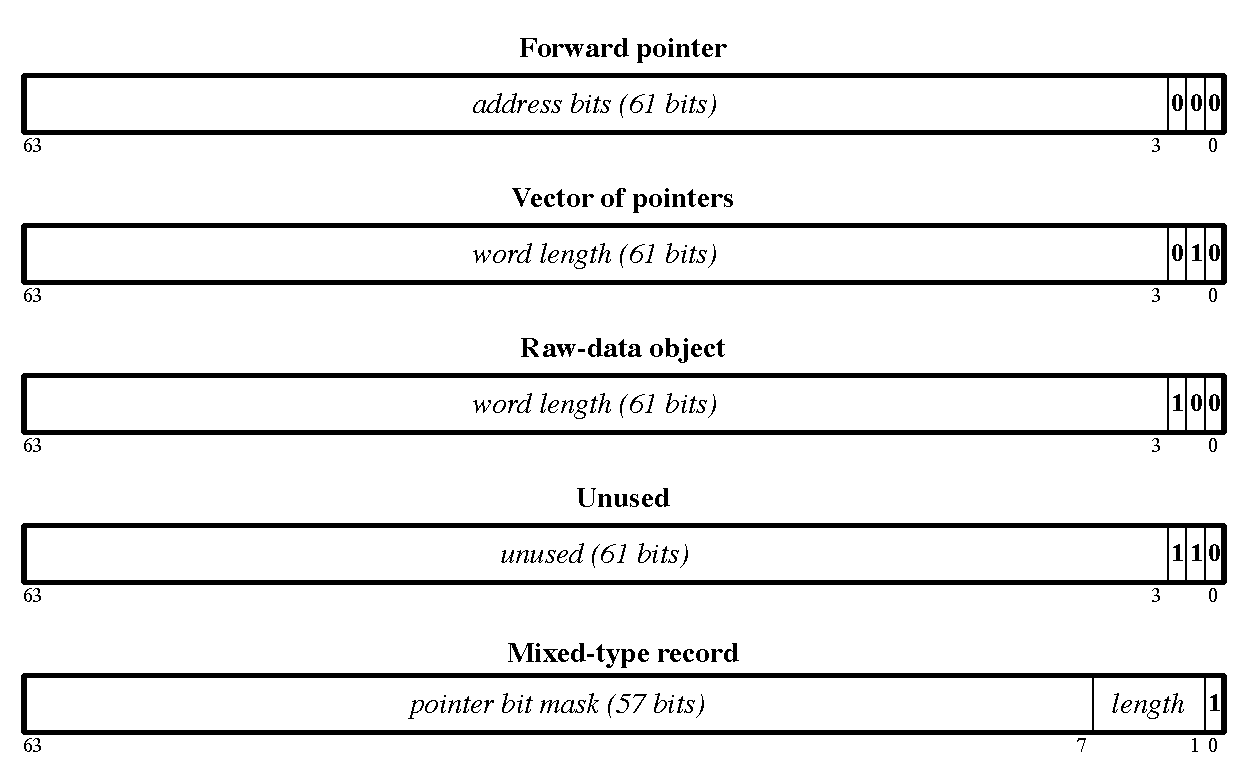
\includegraphics[width=5in]{pictures/old-object-headers}
  \end{center}%
  \caption{Old object-header-word layout}
  \label{fig:old-object-headers}
\end{figure}%

\section{Proposed object headers}
The current header scheme suffers from the lack of expandability.

Proxies, mutable vs. immutable, atomic.

\end{document}  